\mychapter{Premières activités}{cap:premieres-activites}
\lhead{Premières activités}

Cette deuxième section est dédiée au compte rendu de mes activités et de mon apprentissage faits pendant cette première période dans l'entreprise. Celle-ci intègre ma prise de connaissance du fonctionnement global de la structure, avec l'exposition dans l'état des premiers projets qui m'ont été confiés.  

\section{Prise de marques}

Une grande partie de mon apprentissage pendant ces deux premières semaines s'est dévouée à la considération et à l'intégration du fonctionnement informatique et humain de la structure. Connaître l'environnement logique et opérationnel de son infrastructure est fondamental pour initier une perspective de travail. À contrario de travailler seul, sur son propre équipement, pour son intérêt personnel.

%Avant de pouvoir travailler dans une infrastructure, il est fondamental de connaître son fonctionnement logistique \& opérationnel avant d'initier une procédure de mise en oeuvre.

\subsection{Découverte du fonctionnement de l'infrastructure}

Le service technique comporte les techniciens informatique, les administrateurs systèmes et réseaux \& son directeur technique. Les techniciens informatique sont davantage sollicités pour la manipulation ou l'installation d'appareils chez les clients ou dans les datacenters, ainsi que pour le support et la réparation de matériel.
\\ \\
Les administrateurs élaborent le déploiement de ces équipements, planifient leur maintenance et les administrent depuis le NOC. Le directeur technique orchestrant l'ensemble de ces activités, en plus de travailler comme administrateur systèmes \& réseaux de longue date. Les alternants se formant à prochainement devenir des administrateurs systèmes et réseaux.
\\ \\
Les tâches de chacun vis-à-vis des clients sont définies et expliquées dans des \textbf{bons de travaux}, avec des \textbf{bons de livraison} lorsqu'une installation d'équipement doit être faite. Les devis, facturations, gestion des clients et des prospects sont fait par Mr. Pierre-Sala Éric.
\\ \\
À notre arrivée, des \textbf{fiches de postes} ainsi que des cahiers des charges nous ont été confiés pour nous encadrer dans les projets attendus et notre alternance. Ces fiches sont aussi présentes chez les autres corps de métiers pour encadrer leurs activités.

% dire que ces deux premières semaines on a beaucoup questionné sur les hyperviseurs, le réseau...

%réu exploit + technique; comment l'organisation se fait (prestations, bons de travaux, bons de livraisons, devis, fiches de postes); nos accès; noc; hyperviseurs esxi; réseau d'un "datacenter"; prise de connaissance des bonnes pratiques

\subsection{Accoutumance aux bonnes pratiques}

Chaque entreprise a ses habitudes dans son fonctionnement, via leurs applicatifs ou leur méthodologie (gestion des documentations, de l'archivage, des applicatifs, des sauvegardes)... Cela peut aussi s'appliquer à la nomenclature des systèmes, l'arborescence des fichiers... Il m'a paru essentiel d'assimiler les bonnes pratiques de l'entreprise pour m'y intégrer au mieux : le travail y sera plus agréable pour moi et pour les autres.
\\ \\
Ainsi, à mon arrivée, une fiche d'intégration m'a été distribuée avec mes premiers identifiants de connexion pour les applicatifs communs. J'ai ainsi compris par déduction que le nom des sauvegardes, la rédaction des procédures ou la nomenclature des hôtes étaient réglementées et normalisées : je m'y suis tout de suite adapté.
\\ \\
D'autres domaines comme des astuces ou des coups de pouces n'étaient pas explicités. Je les ai découvert notamment lors d'explications de mon travail aux autres personnes de l'équipe, lorsque celles-ci m'expliquaient comment j'aurais pu simplifier mon travail en effectuant des actions différemment avec certains outils. L'accoutumance à une entreprise passe aussi par une bonne prise en main de ses outils.
\\ \\
Cette accoutumance aux applicatifs, aux astuces de certains logiciels ou autres manières de réfléchir à son travail m'ont beaucoup aidés à prendre mes marques les premières semaines.

\section{Mise en place de services internes}

Pour la première prise en main de l'infrastructure, le cahier des charges demandait l'installation de solutions pour l'amélioration, la simplification ou l'ajout de fonctionnalités au travail général de l'équipe d'ADITU. Ainsi, sans avoir à toucher à la criticité de l'infrastructure des clients, j'ai mis en place plusieurs services internes à ADITU.

\subsection{Aménagement d'un environnement conteneurisé}

Les services reposent sur un environnement conteneurisé Docker. Cela minimise les ressources nécessaire par service, augmente la reproductibilité et l'ensemble des solutions devient plus flexible. Pour simplifier la manipulation des ressources Docker (conteneurs, images, volumes, réseaux), une interface graphique intuitive a été montée, permettant le dépannage rapide des solutions - redémarrage en un clique, diagnostique rapide par indicateurs lumineux...
\\ \\
L'ensemble de cette solution repose sur une machine virtuelle \textit{VM}, hébergée sur un hyperviseur.

\subsection{Installation d'un proxy inverse}

L'ensemble des services ont été montés derrière un proxy inverse \textit{reverse proxy}. Un proxy normal permet la centralisation des points de sortie web pour Internet, pour les faire passer par un uniquement équipement. Utile pour restreindre l'accès à certains site, permettre la mise en tampon de pages web entre utilisateurs, ou pour la rétention d'activités globales sur le web.
\\ \\
Le proxy inverse permet la centralisation des accès et le déploiement de plusieurs services derrière une machine avec la même adresse IP. Le principe est identique au proxy simple, mais dans l'autre sens : au lieu de centraliser les points pour sortir vers Internet, il démultiplexe l'arrivée pour les services voulus. Selon le lien \textit{URL} contacté, le proxy inverse redirige l'activité pour le service voulu, en ayant toutes les URL dirigeant vers la même adresse IP.

\begin{figure}[H]
    \centering
    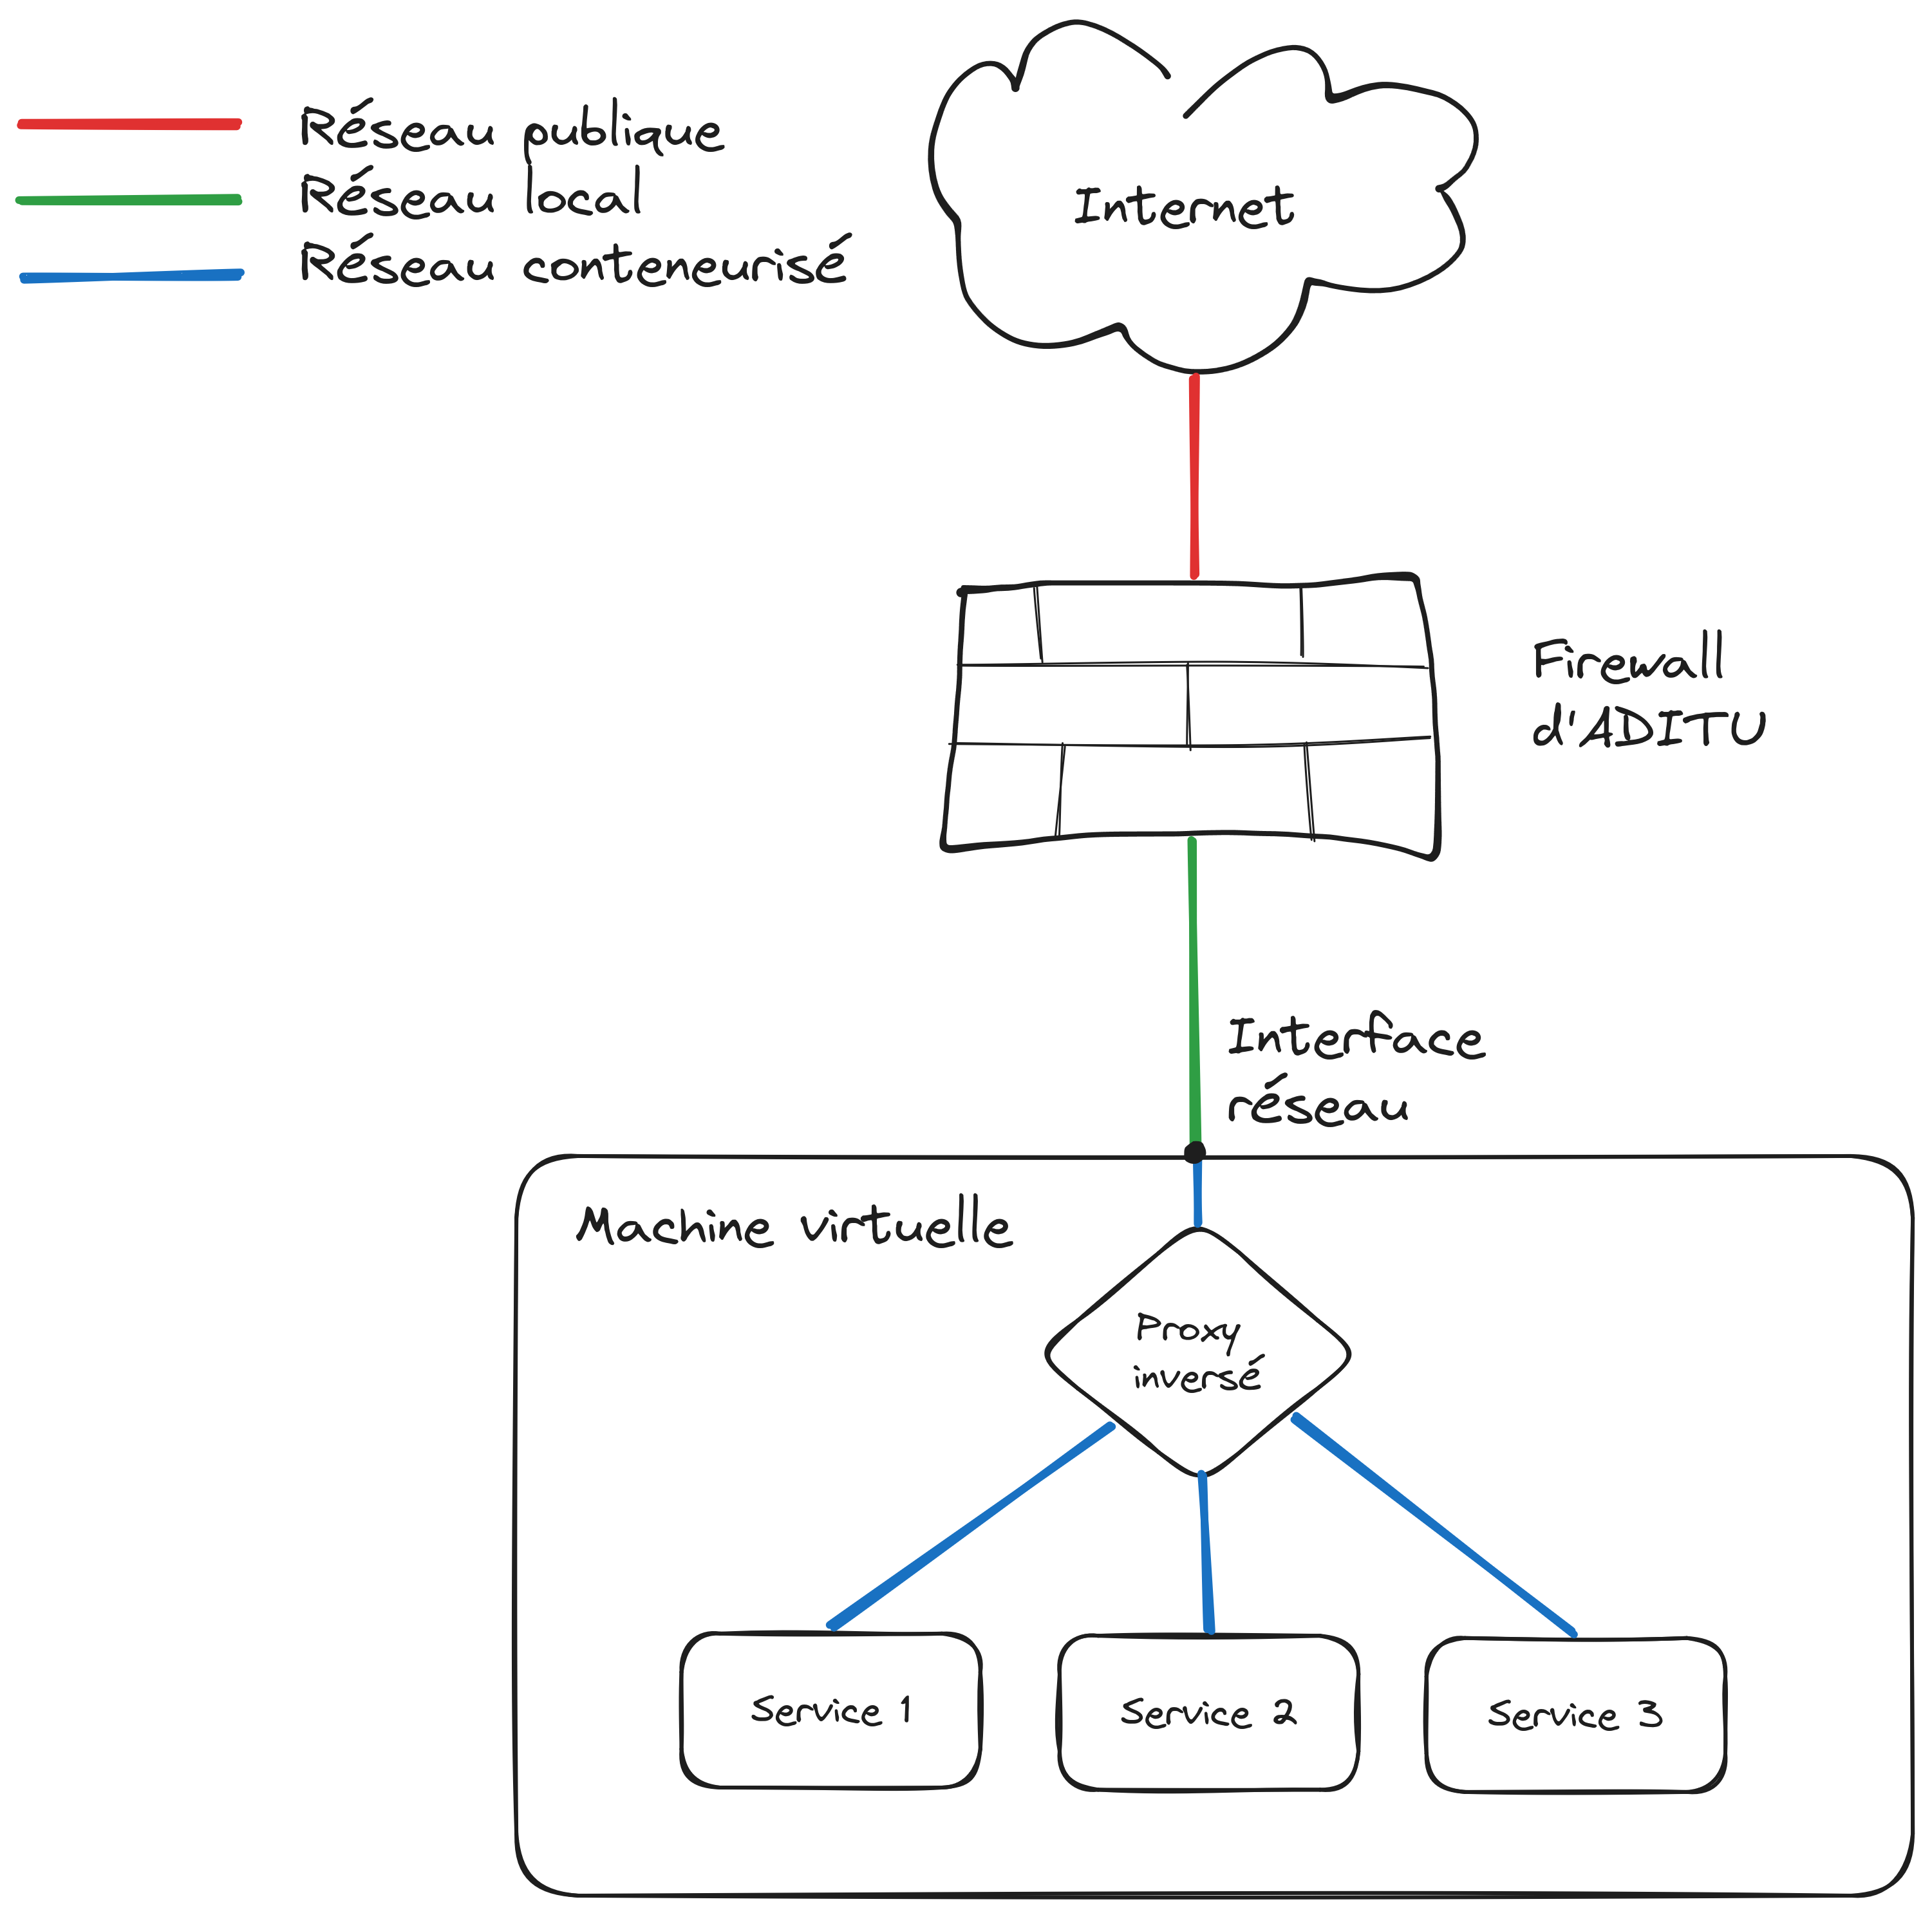
\includegraphics[width=\textwidth - \textwidth / 6]{Untitled-2024-01-21-1259.png}
    \figurename
    \caption{Vision d'esprit simplifiée du proxy inverse}
    \label{fig:rvproxy}
\end{figure}

\noindent Cette manipulation permet l'hébergement de plusieurs services, par communication sur le même port, en n'utilisant qu'une seule adresse IP publique - précieuse car chères à l'achat. La différenciation du service voulu s'effectuant par l'identification de l'URL renseigné.
\\ \\
Le proxy inverse gère les certificat SSL/TLS pour les services qu'il redirige (la sécurisation du traffic), ainsi que le contact des ports. Les services peuvent être hébergés sur une autre machine, à condition que le proxy inverse puisse la contacter sur le port pour communiquer avec le service hébergé.

% explication utilité reverse proxy pour ce qui va arriver après (une ip publique); schéma; donner le nom de la solution

\subsection{Montage d'un service de partage d'informations sécurisé}

Le premier service monté derrière le proxy inverse fut un service de partage d'informations sécurisé. Celui-ci prend place lors d'échange de mots de passe ou de lignes de configuration avec des clients. ADITU peut en envoyer aux clients comme l'inverse.
\\ \\
Au lieu d'envoyer des mots de passe ou des fichiers de configuration par mails, ceux-ci sont regroupés sur une plateforme accessible par l'attendu uniquement (authentification + autorisation). Cette plateforme permet la non divulgation d'informations sensibles par mail (mots de passe, informations sensibles...), leur chiffrement et un accès sécurisé.
\\ \\
Des mesures de sûreté sont mises en place : possibilité de suppression de l'information après première lecture, confirmation de la lecture, temps limite d'accessibilité à la ressource (utile pour les mots de passe qui "ne doivent pas trainer").
\\ \\
Une solution similaire de secours est aussi mise en place. La première étant traduite en français pour un usage primaire et globale.

%mots de passe et fichier de conf

%expliquer pourquoi besoin de ne pas donner mot de passe en clair dans message (un mec vient, récupère; si self-host, un mec vient, galère et par chance abandonne); envoi de fichiers de configuration par yopass; partage avancés de mots de passe pwdpush (voir si personne à vu et quand, temps maximal, accès une fois)

\subsection{Implémentation d'une solution de partage de fichiers volumineux}

Aucune solution de partage de fichiers volumineux n'était présente chez ADITU. Ainsi, le transport manuel ou par hébergeurs tiers étaient nécessaire pour le transfert de fichiers lourds (fichiers compressés, export de boites mail, enregistrement de caméras...).
\\ \\
Une solution de partage de fichiers volumineux a été monté derrière le proxy inverse pour permettre à ADITU et à ses clients de pouvoir y déposer des fichiers \& de pouvoir les partager. Cette solution est davantage professionnel, plutôt que de passer par des services tiers (Google Drive, Microsoft OneDrive...). De plus, celle-ci est hébergée chez ADITU et bénéficie de la sécurité \& la gestion de son réseau.

\subsection{Déploiement d'une console de vérification de disponibilité}

Le centre de donnée de Dax est certifié ISO 27001 HDS pour l'hébergement de données de santée (pour les hôpitaux...). Cette certification demande des tests périodiques de bascule de réseaux d'opérateurs (accès à Internet) et de restauration de sauvegarde.
\\ \\
Le test de bascule d'opérateur revient à simuler la coupure d'un lien vers Internet pour s'assurer que le datacenter soit toujours accessible depuis l'extérieur en basculant sur un lien de secours - haute disponibilité. Pour s'assurer du bon fonctionnement du test de bascule d'opérateur, une console de vérification de l'état des services a été montée, toujours derrière le proxy inverse.
\\ \\
Cette console vérifie en temps réel la disponibilité des services hébergés dans le datacenter de Dax depuis celui de Bidart. Ainsi, lors de la bascule d'opérateur à Dax, les services sont indisponibles pendant un très court instant pendant que les équipements du datacenter adapte leur configuration pour la nouvelle route - selon l'activité, indistinguable par l'utilisateur.
\\ \\
Le rôle de cette console est de superviser la disponibilité des service hérbergés à Dax, utile lors du test de bascule pour vérifier l'accessibilité des services depuis l'extérieur.

% expliquer pourquoi besoin de se simplifier et pas à avoir à génerer des accès à chaque fois; fichier de conf importants parfois mots de passes dedans ou informations sensibles